% vim:set et sw=2 ts=4 tw=72:
\chapter{Background and Related Work}\label{chap:background}

A version control system tracks files, and how that information changes over time.
While it can be used for storing any digital information,
version control is usually used in the context of software development;
it is used for storing and managing the information about
the project, the source code, and the binary assets.
Version control has two primary purposes,
first as a means of storing information,
and second as a means of retrieving historical versions of that information.
In addition to fulfilling the two primary purposes, modern version
control maintains a log of who is making the changes and when the
changes were made.

Early version control systems, such as revision control system (RCS),
were designed for local development and provided no means of collaboration.
As software projects grew, the model quickly became outdated,
being replaced with a centralized server model.
Concurrent Version System (CVS) and Apache Subversion (SVN) are two
examples of centralized version control systems. The centralized version
control system provides means of collaboration through a client-server
interface. The repository is stored in a central server. Developers use
a client to check out parts of the repository, choosing parts that
pertain to the part they are editing.

In large open source projects, the centralized architecture becomes a
burden. Common tasks such as committing and changing branches requires
re-synchronization with the central server.
To work with the repository,
the developer must always have access to the central server.
To maintain the atomic properties of committing, the server will
momentarily lock the repository to ensure that no changes happen while a
commit is being processed or a conflict resolved.

Due to the limitations of a centralized architecture, the Linux kernel
uses a distributed version control system. Until April of 2005, the
kernel project used BitKeeper.
In April 2005, the licensing became too restrictive and Linux was forced
to change version control systems.
Git was written as the replacement for BitKeeper, and was designed to
maintain a similar level of patch granularity as in BitKeeper\footnote{
  initial announcement of git on the mailing list
  \url{https://marc.info/?l=linux-kernel&m=111280216717070}}. The first
version of git was roughly 1300 lines of code and was written and
self-hosting in less than two weeks\footnote{From the git mailing list
  \url{https://marc.info/?l=git&m=117254154130732}}.

BitKeeper is a distributed version control system (DVCS).
In distributed version control, the entire repository is mirrored on
the developer's local computer instead of copying parts of the project.
As a result, the local copy is much larger on disk than with a
centralized repository, but the developer has the freedom to make
changes to the code and to the
structure of the repository without needing to re-synchronize with a
central server.

It is often desirable to have the features of version control available
before a feature is ready to be made public, specifically in the case
where many possible implementations may exist.
It is also desirable that the commits into the master branch of the
master repository leave the project in a state that will both compile
and operate correctly.
Distributed version control makes this possible; developers can combine,
split, and edit commits locally before pushing their changes into the
central repository.

When the developer makes a copy of a non-local repository, this is
called cloning.
The non-local repository is known as the origin repository.
When changes are made to the origin repository, the local clone must
resynchronize with origin in order to for those changes to be propagated.
This resynchronization can be done in one of two ways.
The normal way of resynchronizing is through the \textit{pull} command,
which fetches the changes in the origin repository, then merges the
branches of the origin repository into the corresponding branches in the
local repository.
The second way of resynchronization breaks the process into two steps,
manually issuing the fetch command and then manually merging or rebasing
branches.
Rebasing is the process of moving one or more commits from one ancestor
to another.
The process of updating the origin repository with the changes made in
the local repository is known as pushing.
If there are no merge conflicts, the merge can perform a fast-forward
merge, shown in Figure~\ref{fig:fast_forwarded_merge},
which flattens the changes made in the origin repository into the
master branch of the local repository.
Fast-forward merging hides the fact that git would otherwise consider
the two repositories to be separate branches.
Without fast-forward merging, any resynchronization would result in the
addition of a new merge node.
If there is a merge conflict, or the user has specified that the merge
should not fast-forward, a merge commit is created, as shown in
Figure~\ref{fig:merge_node_merge}.

\begin{figure}[htpb]
  \centering
  \begin{subfigure}[b]{0.5\textwidth}
    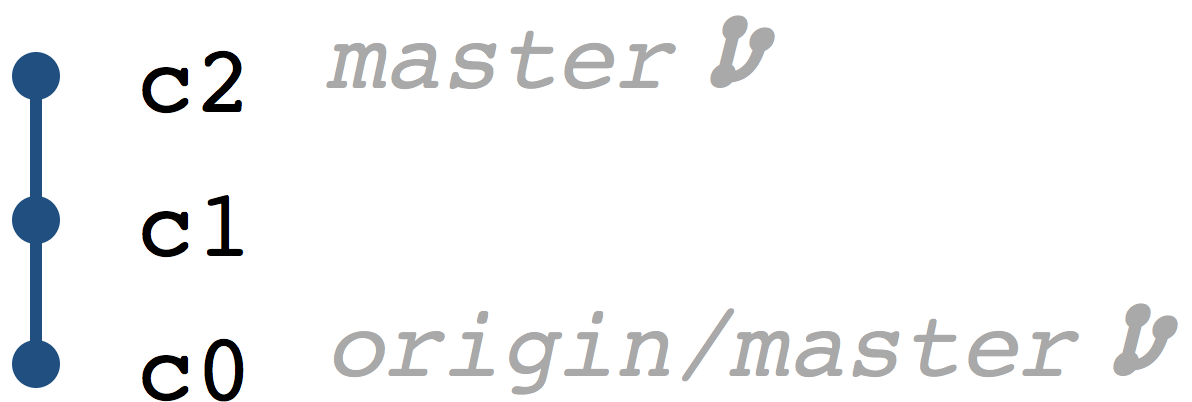
\includegraphics[width=0.85\textwidth]{Figures/background/repos/base_repo.png}
    \caption{Example of a basic repository where the local master branch
      is two commits ahead of the origin master branch.}
  \end{subfigure}

  \begin{subfigure}[b]{0.5\textwidth}
    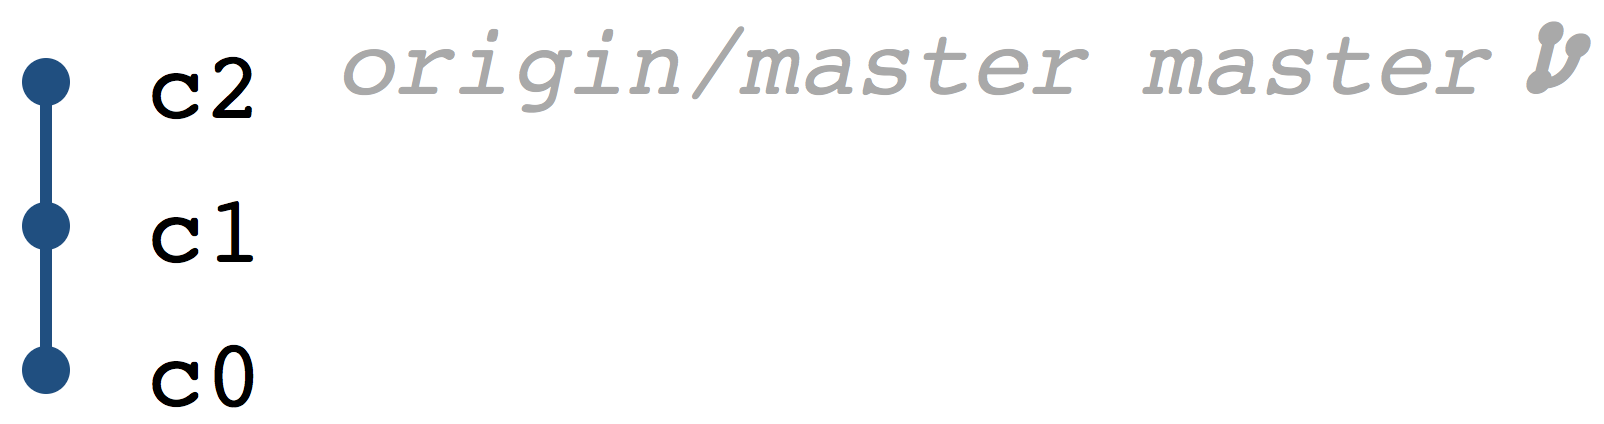
\includegraphics[width=\textwidth]{Figures/background/repos/fast_forward.png}
    \caption{The fast-forward merge moves the origin branch pointer to
      the current master}
    \label{fig:fast_forwarded_merge}
  \end{subfigure}

  \begin{subfigure}[b]{0.5\textwidth}
    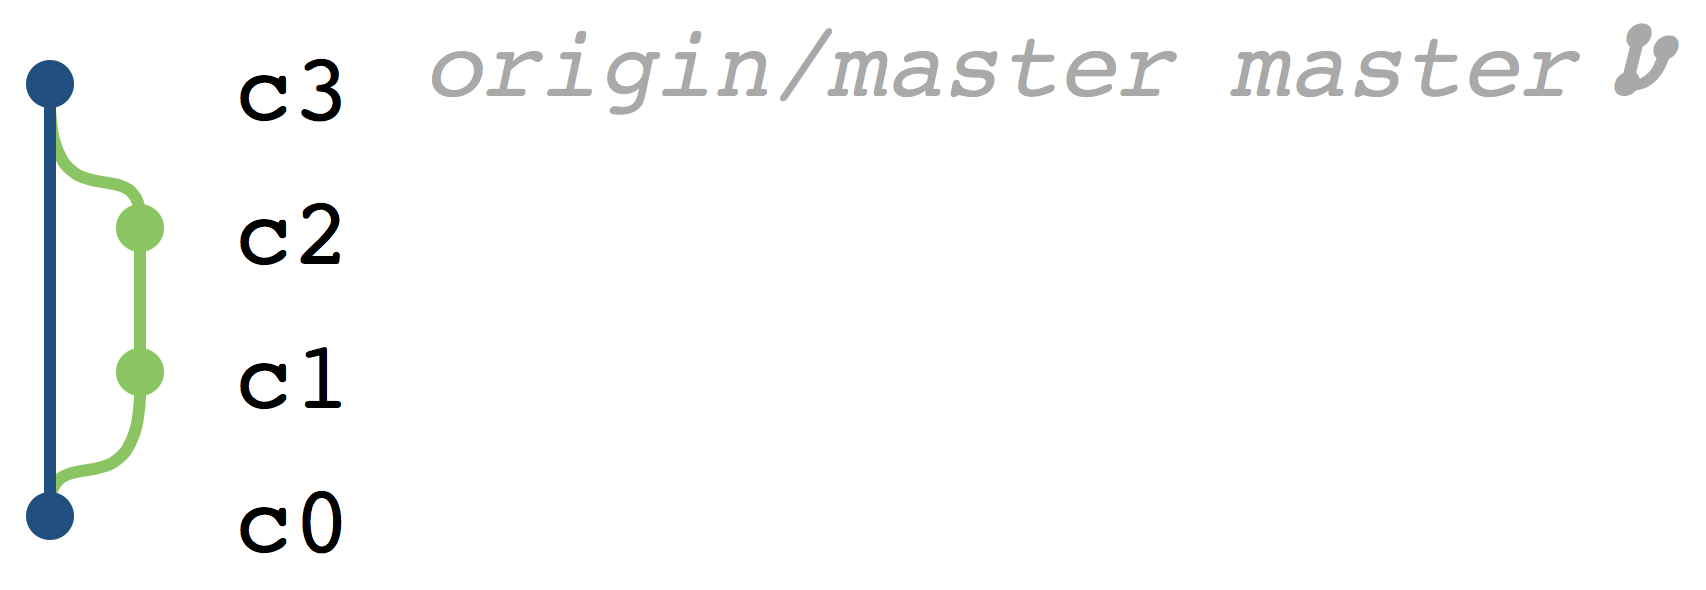
\includegraphics[width=\textwidth]{Figures/background/repos/merge_commit.png}
    \caption{A merge node is created when the merge cannot be made
      cleanly, or \textit{--no-ff} is passed to the merge command.}
    \label{fig:merge_node_merge}
  \end{subfigure}
  \caption{The distinction between fast forward and non fast forwarding
  merges is shown}
  \label{fig:merge_styles}
\end{figure}

Git is an implementation of a distributed version control system.
Distributed version control gives developers more flexibility with their
local repository and requires the developer to synchronize their local
copy of the repository with the public master repository less often
than with centralized version control.
The public master repository can be thought of as being the equivalent
of the central repository in a centralized system.
Instead of it being enforced by the version control system,
it is a socially agreed upon location where the official version of the
code exists.
Unlike with the centralized version control though,
there is no requirement for the developer to ever push their changes
back to the public repository;
the local repository is completely standalone.
Because the local repository is separate, the developer has more
flexibility to alter the structure of the repository before pushing
the results back into the master repository.

With the additional flexibility, the structure of large and active
repositories is more complex than the repositories that are in
centralized version control. This poses a problem for a maintainer who
must understand how a commit is integrated into the master branch of a
project and the other commits that are integrated with that commit.
Maintainers must sift through thousands of commits to determine which
changes being made to the current version of the software pertain to
the area of the software that they are maintaining.
Specifically, maintainers must be able to answer two questions:

\begin{textbox}
\begin{itemize}
  \item How is a commit integrated into another branch?
  \item What other commits are integrated with the commit?
\end{itemize}
\end{textbox}

The remainder of this chapter includes related work, a description of
git, the directed acyclic graph used internally by git, and information
about the Linux kernel repository.

\section{Related Work}\label{sec:related_work}

A Version Control System (VCS) tracks the development of a software project,
recording each change as it happens. By tracking the changes, the VCS
contains an entire story of the software, rich with information about
who the authors are, what files are being modified, what where changes
are being made. This makes the VCS vital in providing information about
how a software project is being developed and how the software is
structured. In order to use the information stored in the VCS, users
must be able to gain a clear understanding and summarization of the
changes being made, and how they interact with the rest of the source
code. While there has been extensive research on visualizing software
repositories, previous work does not focus on how commits and merges are
structures in the repository graph, and in extension, how commits are
integrated into a repository. The literature on repository visualization
and summarization can be broken down into three academic subcategories:
communication\cite{Cubranic2005,Begel2010}, aspect-oriented
visualization\cite{Ambros2005,Burch2005,Ambros2009}, and organic
visualizations\cite{ogawa09,Caudwell2010}. A fourth industrial category
exists, including tools like GitKraken and SourceTree. The goal of the
industrial tools is not to extract or synthesize new information from
the repository, but to act as a user-friendly client on top of what git
already provides.

Many tools focus on addressing the issue of communication between
developers in inter-team collaborative work. Hipikat\cite{Cubranic2005}
investigated communication between developers, focusing on assisting
with the integration of new developers into a project though
communication, providing the new developer with searchable artifacts of
the changes being made, and where to find them. The artifacts may
include files or bug information, shown in Figure~\ref{fig:hipikat}.
Codebook\cite{Begel2010} also focused on communication, but where
Hipikat focused on assisting new developers find artifacts, Codebook
assists developers with finding who was responsible for creating the
artifact. Codebook used a data-mining technique to determine the
developer of a piece of code, the program manager who wrote the
specification for the code, and the program managers and developers on
the team who were working together. A screenshot of Hoozizat, an
implementation of codebook, is shown in Figure~\ref{fig:codebook}.
Hoozizat and Hipikat use the version control as the archive of artifacts
that are being queried. Neither tool is designed with the goal of
providing information on the topological structure of a source code
repository, nor are these tools designed for visualization purposes, but
they do draw information from the contents of the version control
system.

\begin{figure}[htpb]
  \centering
  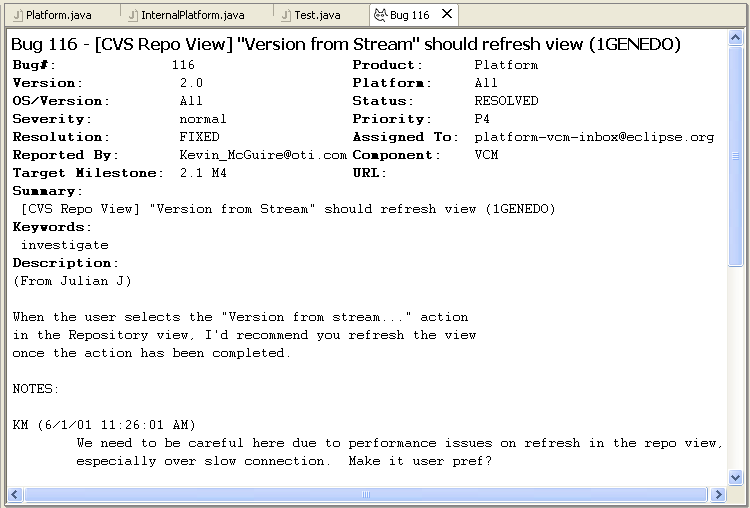
\includegraphics[width=0.9\linewidth]{Figures/introduction/hipikat_bug.png}
  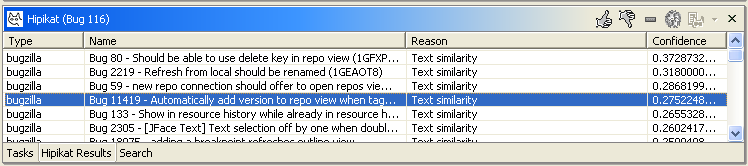
\includegraphics[width=0.9\linewidth]{Figures/introduction/hipikat.png}
  \caption{View of Hipikat, listing bugs that are similar to the one
  being viewed}
  \label{fig:hipikat}
\end{figure}

\begin{figure}[htpb]
  \centering
  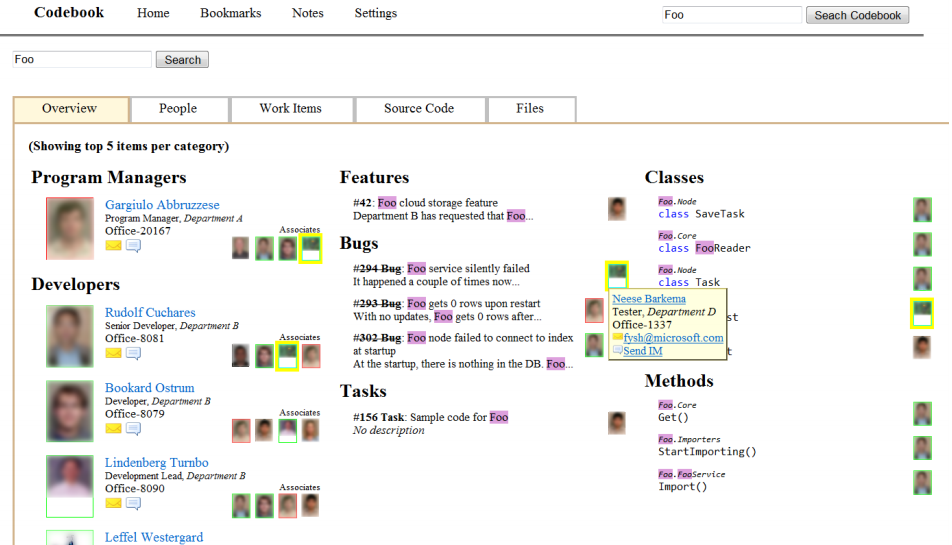
\includegraphics[width=0.8\linewidth]{Figures/introduction/codebook.png}
  \caption{A screenshot of the search results on Hoozizat, an
    implementation of codebook.}
  \label{fig:codebook}
\end{figure}

Most visualization systems provide information about a certain aspect of
the contents in the repository. The goal being Fractal
Figures\cite{Ambros2005} is to show the division of work between
contributors. The project is represented as a square. The square is then
subdivided based on the proportion that a given contributor contributed
to the project, shown in Figure~\ref{fig:fractal_figures}. The
visualization makes it easy to see where work is evenly divided versus
the projects where a single contributor is doing most of the work.

\begin{figure}[htpb]
  \centering
  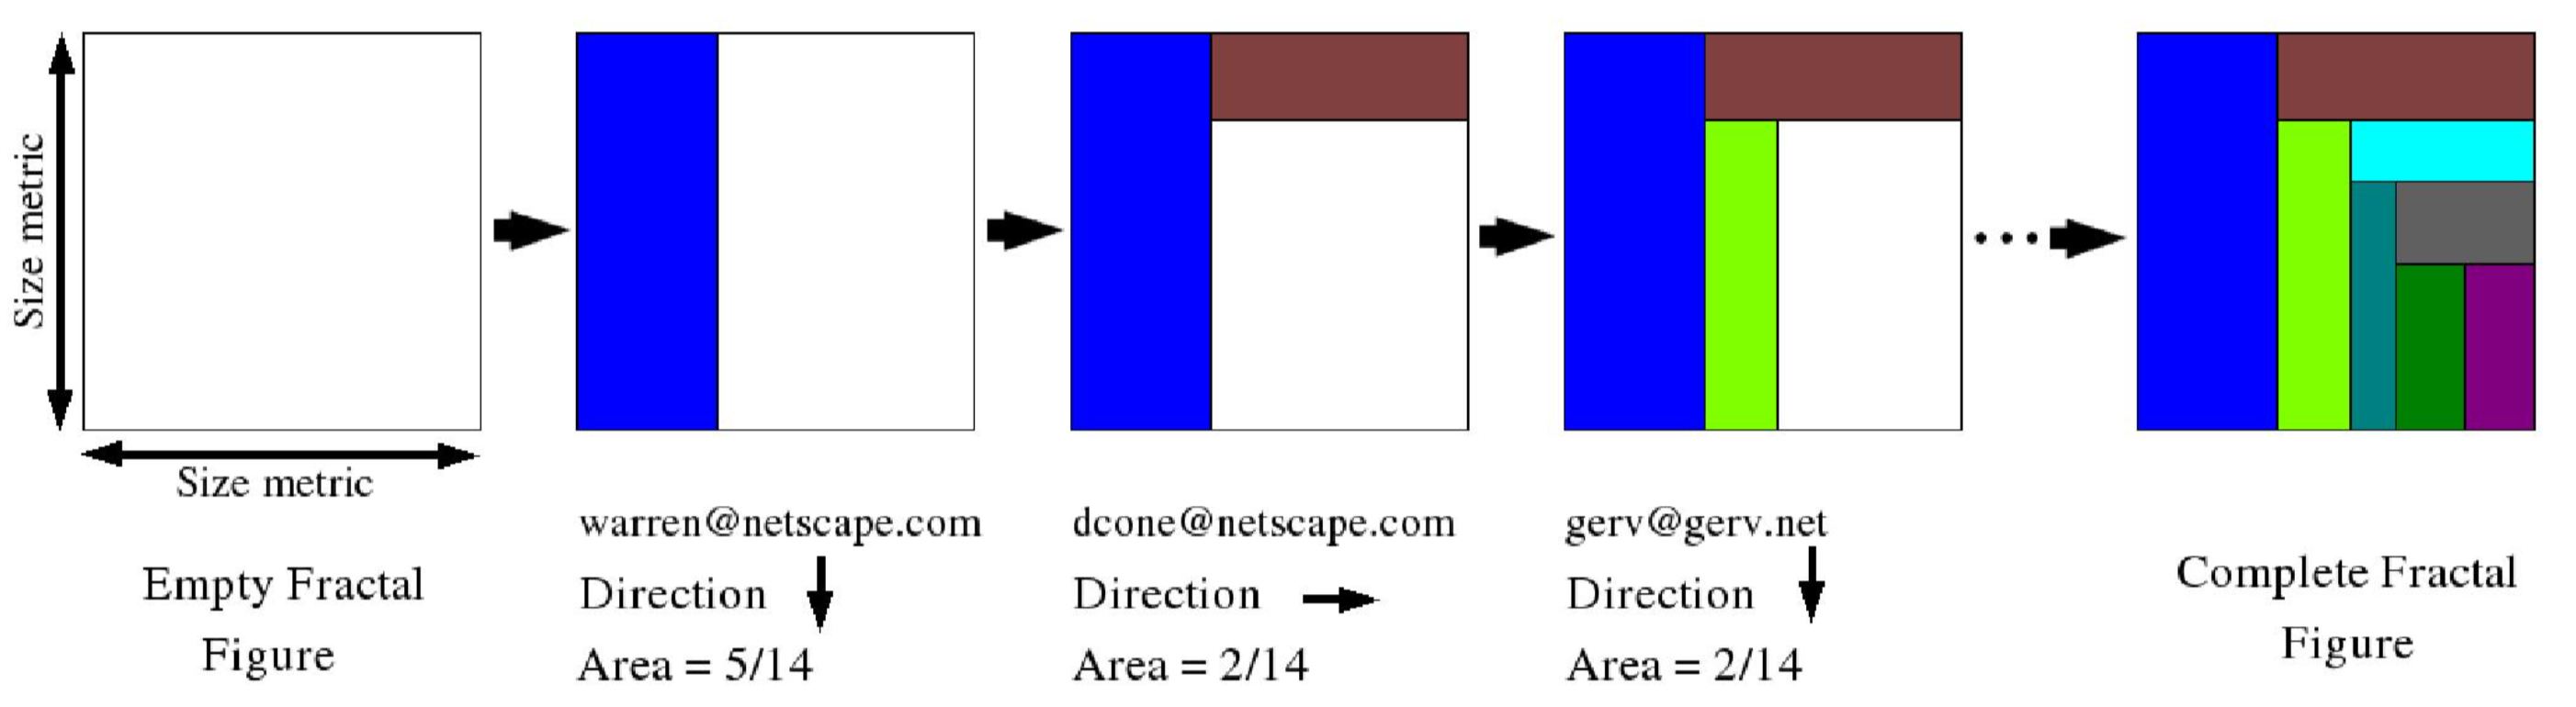
\includegraphics[width=0.8\linewidth]{Figures/introduction/fractal_figures.png}
  \caption{Construction of Fractal Figures}
  \label{fig:fractal_figures}
\end{figure}

EPOSee\cite{Burch2005} and Evolution Radar\cite{Ambros2009} use the
information from the version control to determine which files are edited
together. The tools from these papers are designed to help a user
identify the degree to which two files are coupled. Two files are
edited and committed together frequently are said to be more tightly
coupled. This makes it possible to determine when two classes are
semantically related. The evolution radar shown in
Figure~\ref{fig:evolution_radar} places points on a circle based on the
name and coupled they are. The files are arranged around the circle
based on the file name, including the full file path. This has the
effect of grouping files that are from the same directory. The distance
from the center of the circle is dependent on how tightly coupled the
file is to the file be analyzed. A more tightly-coupled file will be
positioned more closely to the center of the circle.

\begin{figure}[htpb]
  \centering
  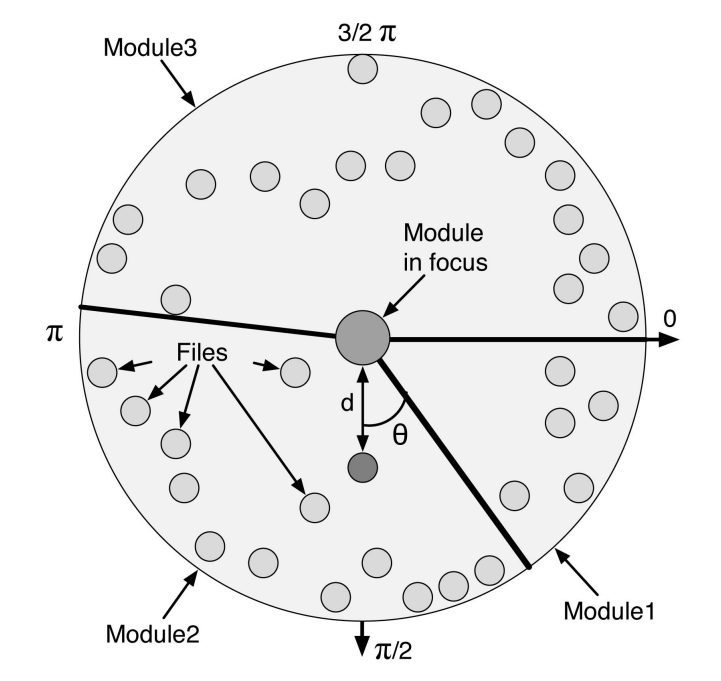
\includegraphics[width=0.8\linewidth]{Figures/introduction/evo_radar.png}
  \caption{Evolution Radar visualization}
  \label{fig:evolution_radar}
\end{figure}

Hoozizat, Hipikat, Fractal Figures, EPOSee, and Evolution Radar all
extract data from CVS repositories. Our goal is to provide information
about git repositories. Fewer tools are available for generating
visualizations and summaries of git repositories, potentially due to the
DAG model used as the internal structure of git repositories.

Organic visualizations show patterns in cooperation and communication
that arise within a software project organically. Heller et
al.\cite{Heller2011} plots communication on a map. This visualization
shows communication and cooperation patterns that arise, and how they
cross country boundaries, within a software project. The visualizations
proposed in Gource\cite{Caudwell2010}, shown in
Figure~\ref{fig:gource_view}, shows which files contributors are working
on. Using this, it is possible to draw conclusion about which parts of a
project a given contributor is working on and the group of contributors
working on a given area. Gource uses a graph metaphor structure to
represent the file structure of a repository. Files in the same
directory cluster together to form a node. Edges between the directory
clusters represent which directory contains another, although there is
no way to determine the direction of the relationship. User avatars move
around the graph emitting different beams of colored light depending on
the change being made to the file. Greed indicates the creation of a new
file, yellow indicates a modification, and red indicates the deletion of
a file. The visualization is animated to show how a project grows over
time. Codeswarm\cite{ogawa09}, shown in Figure~\ref{fig:codeswarm}, is
similar to Gource, using an organic timelapse approach to visualizing
the events in the repository. Unlike Gource, which constructs a graph
from the directory structure of project, Codeswarm does not have a graph
structure; developers are the center of the visualizations. When a
developer makes a change to a file, the file lights up and flies toward
the developer. As a developer makes more changes, the files that the
developer is modifying will form a ring around the developer. If
multiple developers are modifying a file, the developer nodes are drawn
together.

\begin{figure}[htpb]
  \centering
  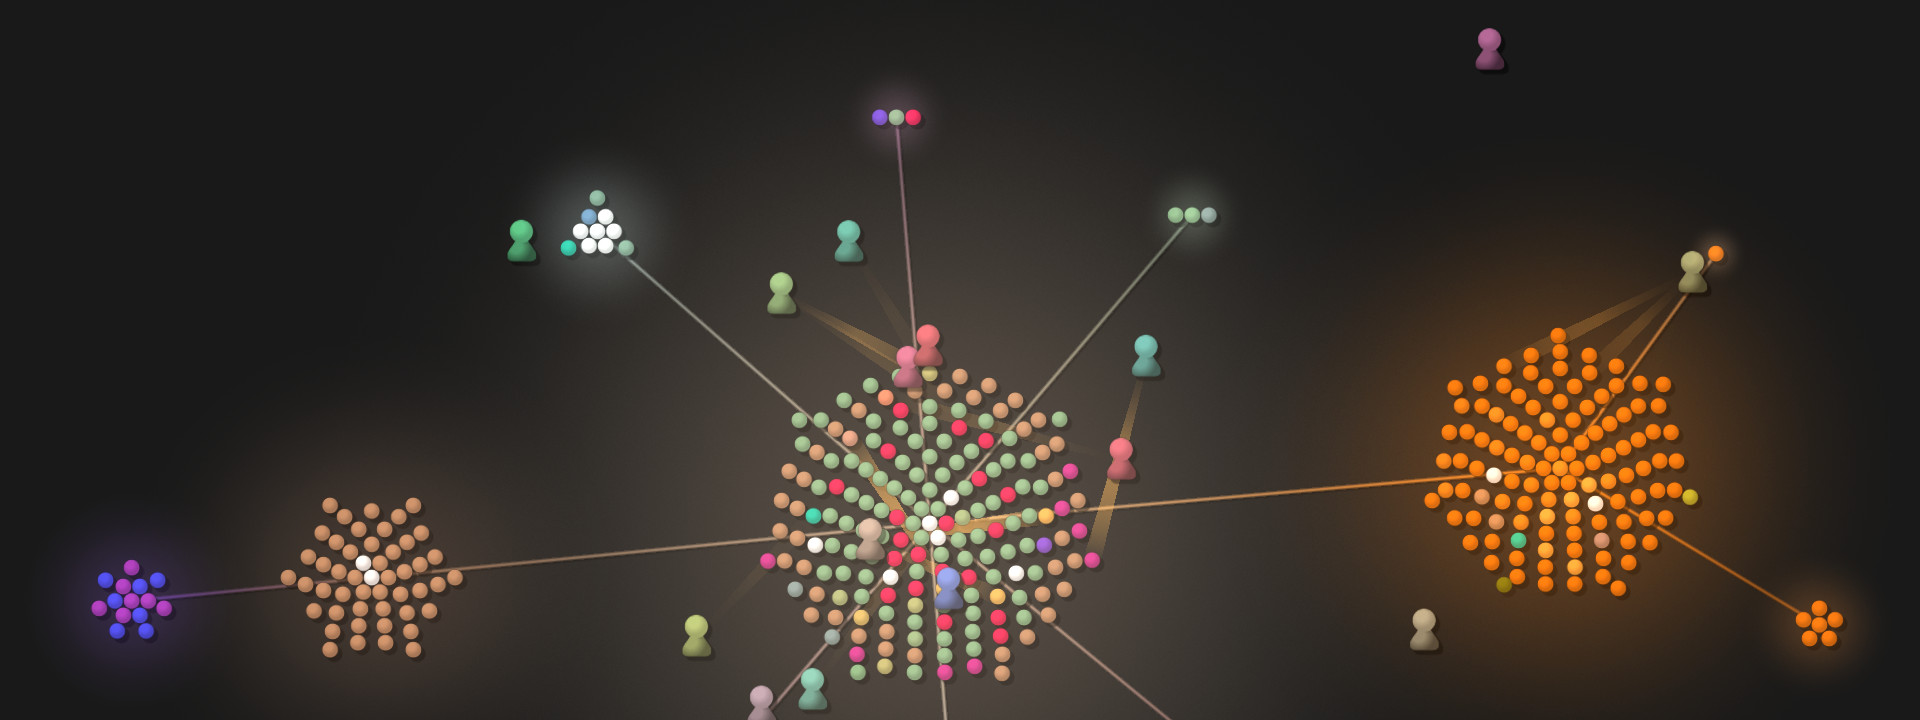
\includegraphics[width=0.8\linewidth]{./Figures/introduction/gource-linux.jpg}
  \caption{View of Gource file graph with users operating on a
    repository}
  \label{fig:gource_view}
\end{figure}

\begin{figure}[htpb]
  \centering
  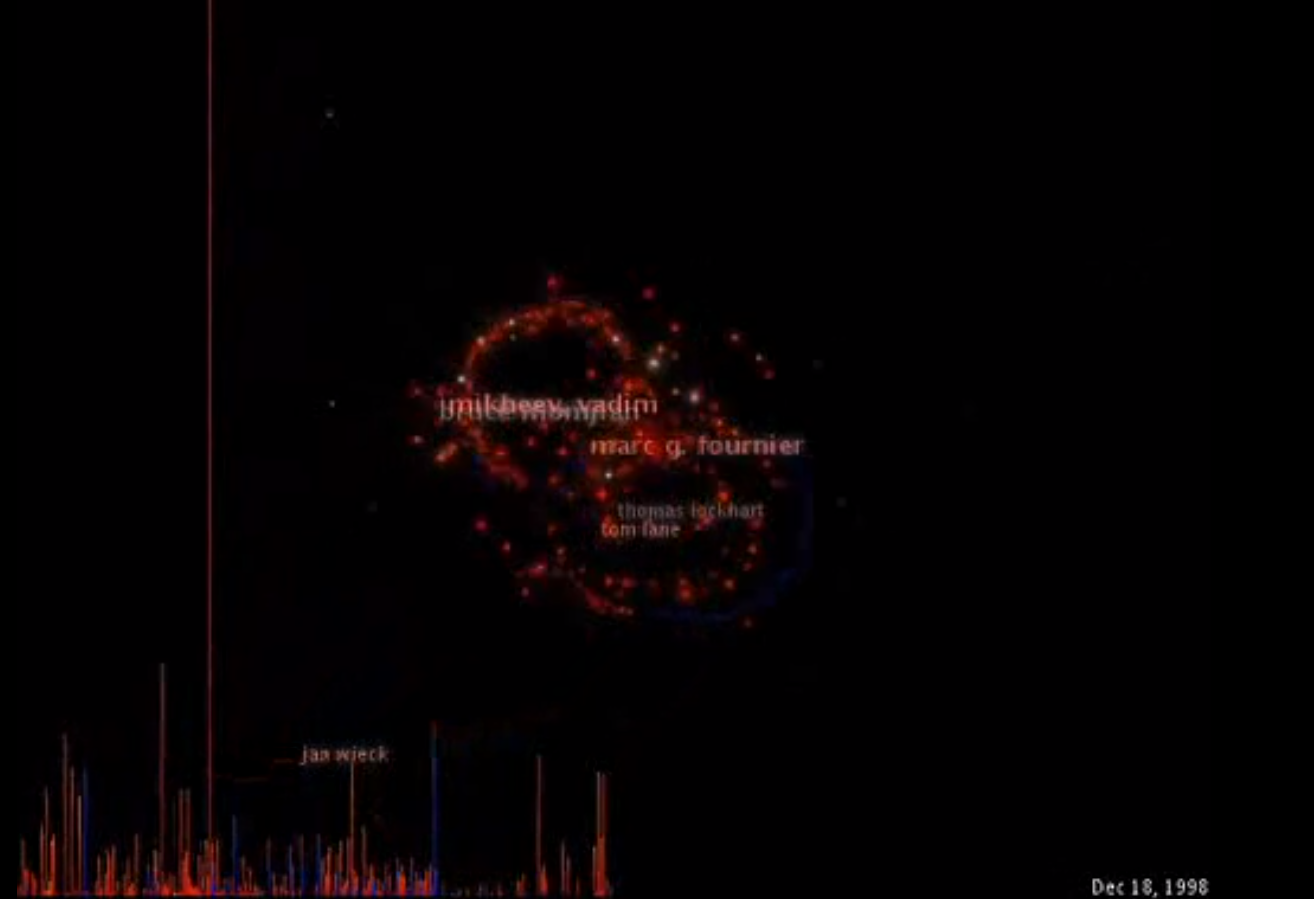
\includegraphics[width=0.8\linewidth]{Figures/introduction/codeswarm.png}
  \caption{View of the Postgresql repository in Codeswarm}
  \label{fig:codeswarm}
\end{figure}

There are many non-academic tools that are designed as an interface to
git. While not all of these programs provide visualizations, those that
do use a visual metaphor of the DAG to show topological information
about the commits in the repository. While they ultimately show the same
information, the topology of the repository, the organization of that
information is different.

GitKraken, shown in Figure~\ref{fig:gitkraken_main},  is a popular
commercially written git interface that aims to be efficient, elegant,
and reliable, according to it's official website. On visual inspection,
it appears to satisfy these goals. Overall, the interface is clean, most
actions that are possible with the git command line are available in the
graphical interface. Overall, the tool is effective and garners online
approval from users. The graph itself, shown in the center of the main
view provides users with the same information as the graph visualization
in gitk and the git command line, though it may be visually more
appealing.

\begin{figure}[htpb]
  \centering
  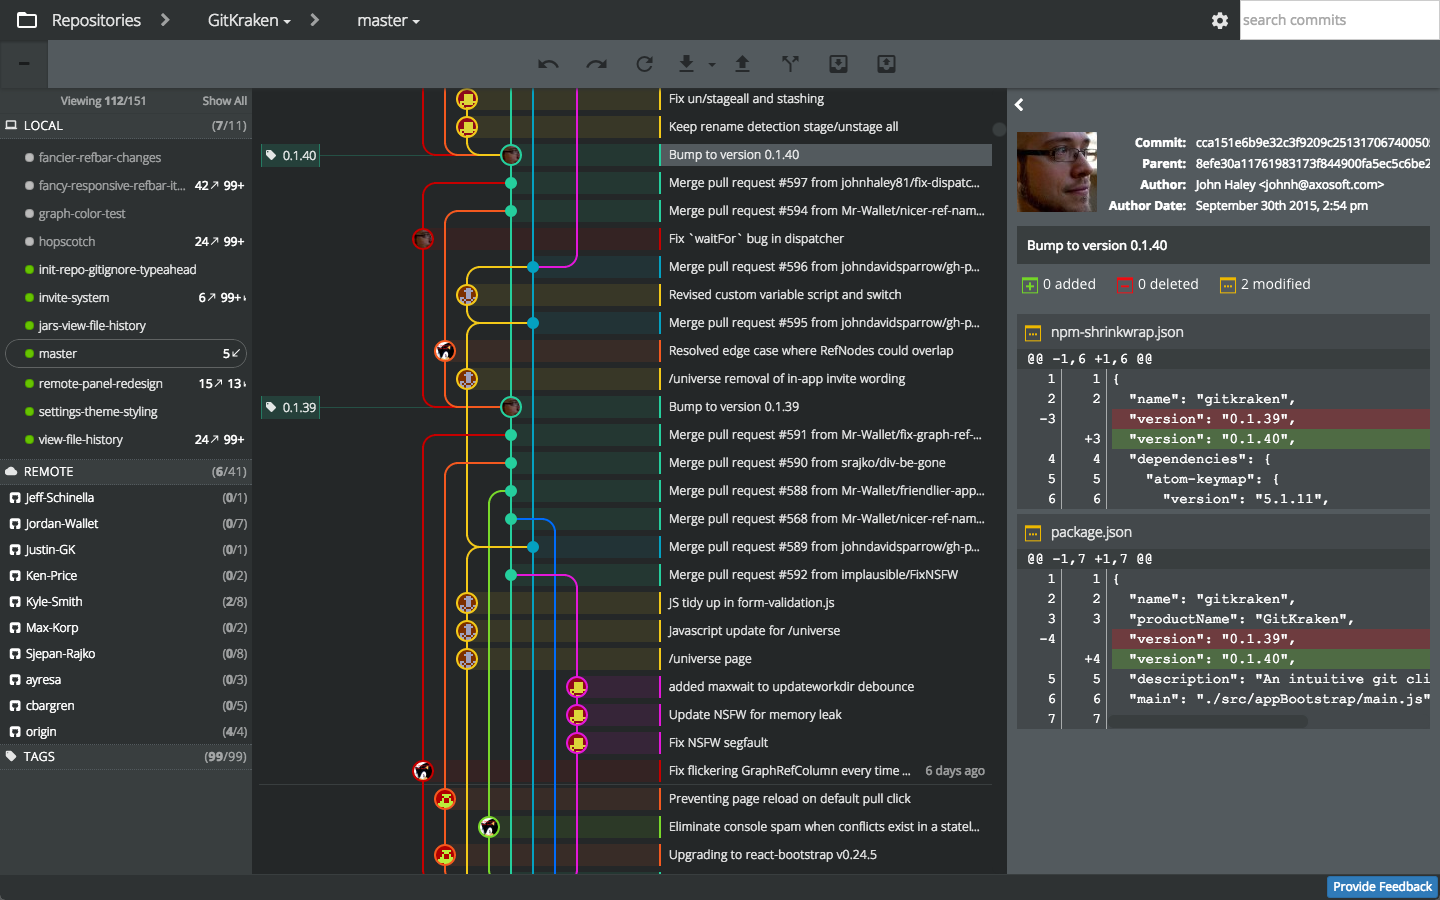
\includegraphics[width=0.8\linewidth]{Figures/introduction/gitkraken_main.png}
  \caption{Screenshot of the main view in GitKraken}
  \label{fig:gitkraken_main}
\end{figure}

In January of 2018, the Gnome project released a replacement for Gitk.
Gitg, shown in Figure~\ref{fig:gitg_screenshot}, is the git GUI client
for the Gnome environment. The visualization is relatively clean, and it
is able to produce a visualization of the Linux repository quickly.
Unlike Gitk, there is no way to navigate to a commit directly using the
commit hash, but the search feature is able to search the repository
quickly without issue. A major drawback in Gitg is that, like in Gitk,
long branches are cut with arrows, but unlike in Gitk, the arrows do not
hyperlink to the other side of the branch. There is no apparent way to
find the other side of the branch without manually looking for it.

\begin{figure}[htpb]
  \centering
  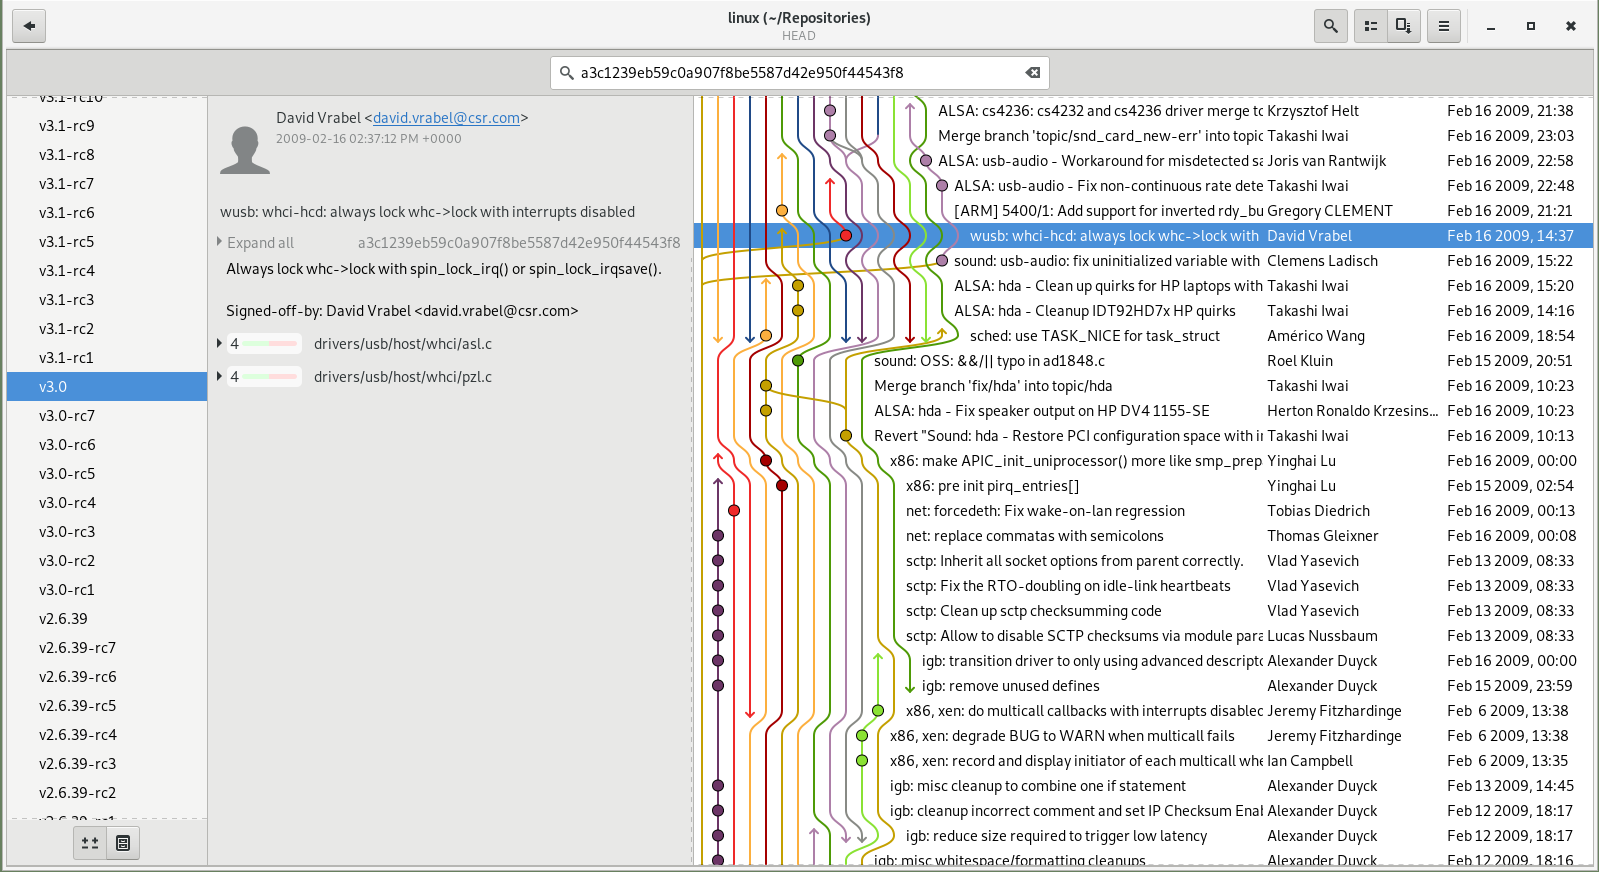
\includegraphics[width=0.8\linewidth]{Figures/introduction/gitg.png}
  \caption{Gitg interface from the Gnome project}
  \label{fig:gitg_screenshot}
\end{figure}


GitLab and GitHub are both online repository hosts, with
visualization and summarization provided as well. While the GitLab
visualization does not appear to provide any additional information, the
visualization provided by GitHub takes advantage of additional internal
knowledge to display information about forks. Through this
visualization, GitHub displays the branch history of the repository
network, including the branches of the main repository and forks from
that. Giteye and most of the other visualizations are relatively
conventional, simply cleaning up the interface of Gitk, the visualizer
that is shipped with git. With the exception of Gitk, no GUI visualizers
are able to produce a visualization for the Linux repository, due to its
size: the GitHub visualizer displays an error message, stating that
there are too may forks to display; the GitKraken interface will freeze
and eventually crash while trying to load the repository; Giteye
and the other visualizers will consume all of the system memory before
they are able to produce a visualization. The Gitk interface is the
least polished, but is able to produce a visualization of the
repository.

\begin{figure}[htpb]
  \centering
  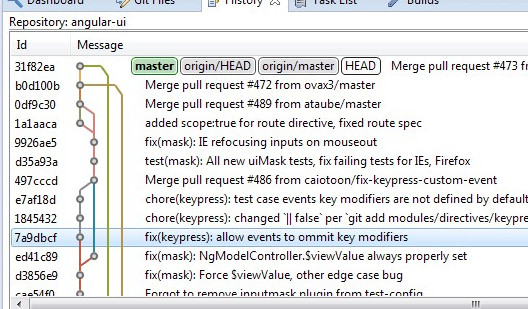
\includegraphics[width=0.8\linewidth]{Figures/introduction/giteye_graph.jpg}
  \caption{Screenshot of Giteye DAG view of a repository}
  \label{fig:giteye_screenshot}
\end{figure}

\begin{figure}[htpb]
  \centering
  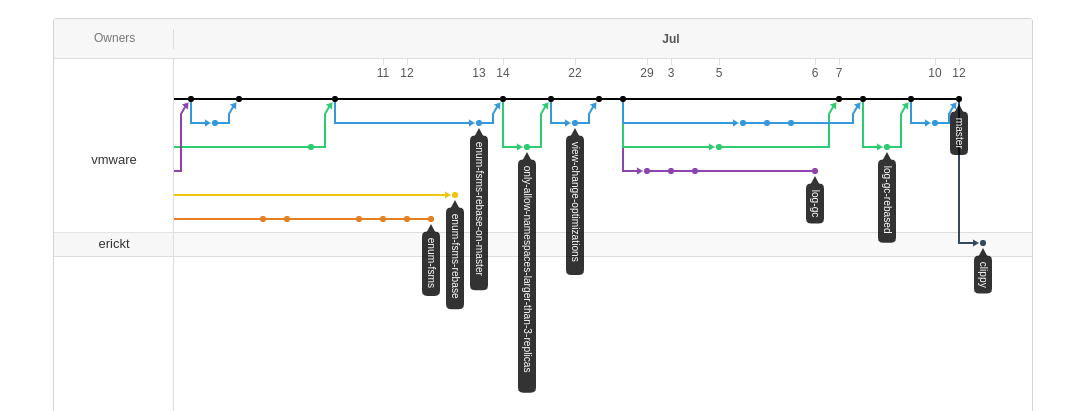
\includegraphics[width=0.8\linewidth]{Figures/introduction/github_dag.png}
  \caption{GitHub online network view of a repository}
  \label{fig:github_dag_screenshot}
\end{figure}

\begin{figure}[htpb]
  \centering
  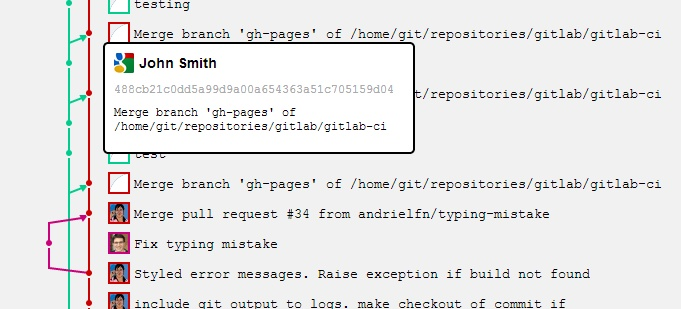
\includegraphics[width=0.8\linewidth]{Figures/introduction/gitlab_graph.jpg}
  \caption{GitLab online graph view}
  \label{fig:gitlab_dag_screenshot}
\end{figure}

\section{Git}
\label{sec:git}

% Commits;
Commits are the most basic unit of change in the git repository.
Commits are how the changes and metadata are stored.
Commits in git are immutable; a commit cannot be changed once created.
Instead, modifying a commit will result
in a new commit with a different commit hash.
Because the commits that follow have references to the updated commit,
those commits are copied and receive a new commit hash as well.
Commits store the commit hash, commit date,
committer, author, and authorship date, the patch, and an ordered list
of parents. The metadata is shown in Figure~\ref{fig:commit_metadata}
for a commit and merge within the repository for this \paper{}.

\begin{figure}[htpb]
  \centering
  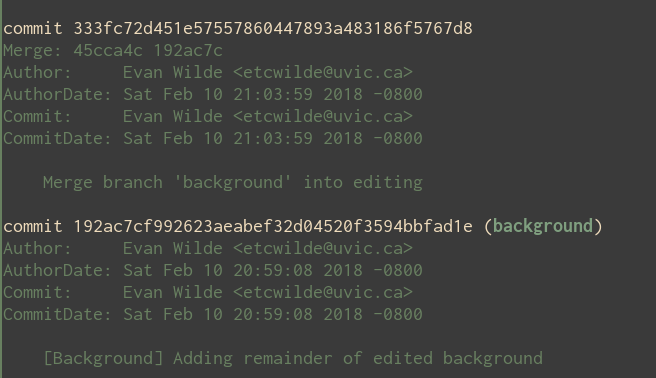
\includegraphics[width=0.8\linewidth]{Figures/background/commit_metadata.png}
  \caption{Screenshot of commit metadate for a commit and merge in the
    repository for this \paper{}.}
  \label{fig:commit_metadata}
\end{figure}

Git allows commits to be made on the behalf of another person, either
via email, or simply because the author of the commit doesn't have the
ability to write to the repository.
When someone else makes the commit, the committer and author will not
match. The patch contains the changes being made, including the
filenames, the line numbers, and the actual change, as shown in
Figure~\ref{fig:commit_patch}.
Rebasing will also change the committer and commit date.

\begin{figure}[htpb]
  \centering
  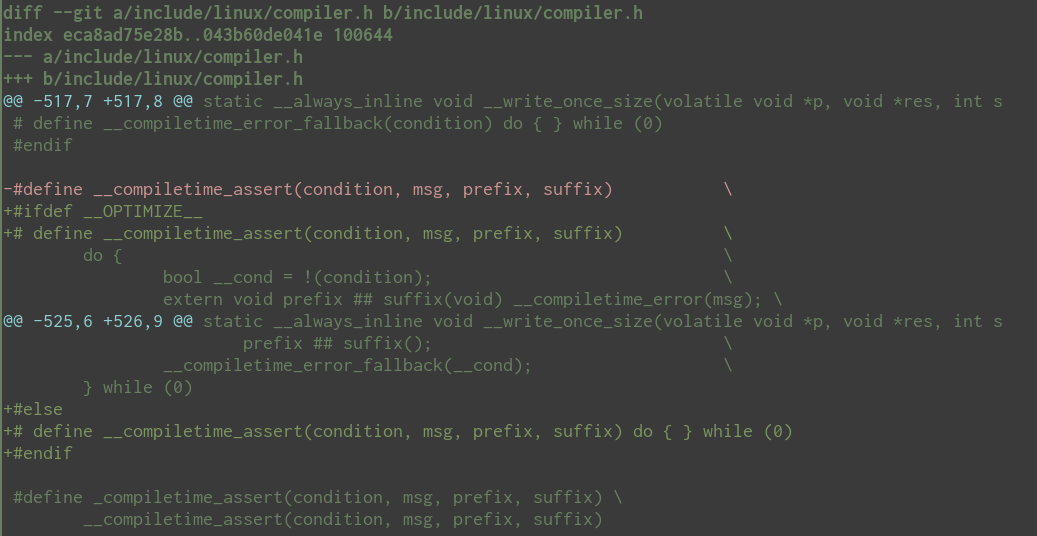
\includegraphics[width=0.8\linewidth]{Figures/background/commit_patch.png}
  \caption{Example of a commit patch from the Linux kernel repository
    from commit \textit{c03567a8e8d5}.}
  \label{fig:commit_patch}
\end{figure}

The parents of a commit are the next commits toward the initial commit.
The first parent in the list is the commit that is on the same branch
as the commit that is being created, i.e, the branch that the other
branches are being merged into.
The remaining commits are the branches being merged, in the order that
they are specified in the merge.
A non-merging commit will only have one parent.
To clarify the difference, non-merging commits are referred to as
commits, merging commits as merges.
In the scope of this thesis, repository event or event is used to refer
to both commits and merges.
The patch are set of changes being made to the files of the repository.

% Integration;
Integration is the process by which the changes in a commit are added to
the master repository.
A small change with few dependencies are easier to integrate than
changes.
It is possible to merge these changes into the master repository
without additional commits making changes.
The changes are directly merged into the master repository.
Many times, these changes are small, localized, bug fixes, or modifications to
documentation, which can be integrated with the rest of the project
without making changes beyond the scope of the bug or documentation.
An example of this from the Linux repository is shown in
Figure~\ref{fig:single_commit_merge}.

\begin{figure}[htpb]
  \centering
  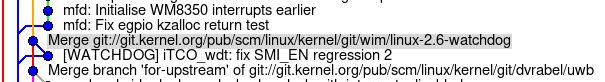
\includegraphics[width=0.8\linewidth]{Figures/background/single_commit.png}
  \caption{Example of a merge that only integrates a single commit}
  \label{fig:single_commit_merge}
\end{figure}


Adding additional functionality to a project may require additional
support from other components of the project.
Non-localized changes may be necessary to provide the additional
information needed for the new function.
Commits can be logically grouped based on the submodule that grouped
based on what part of the project they are modifying.
In the Linux kernel, it is customary to have commits related to
networking in a single merge.
This merge has sub-merges containing wireless networking, Bluetooth,
and Ethernet, among the other implementations of networking.
In this form, the merges act in a similar manner to subdirectories in a
file system, where each directory contains files that work together.

Projects may also be shared between multiple organizations.
The organizations will likely have their own internal master
repositories that they work with before pushing the full set of
changes upstream to the public master repository.
In git, it is possible to merge repositories since they are treated in
the same way as local branches.

In order to integrate the changes, the commits must be merged into the
master branch of the repository.
Commits may be merged directly into the master branch, or may be merged
into multiple branches before finally reaching the master branch.
To understand how a commit is integrated, it is necessary to know which
merges a commit passes through to reach the master branch, and which
commits are merged with it.
Merging commits is the process of integrating them.

Merges are a type of commit; it is possible to make additional
changes while merging.

When two commits from different branches make changes to the same file,
a conflict occurs.
Git is unable to determine which changes are correct, so it flags them
as a merge conflict, which stops the merging process.
The person making the merge decides which change should be kept,
and which should be removed.
The resolution of merge conflicts is stored as the patch of merge
conflicts.
The Linux repository has no merge conflicts.
This is attained through a different workflow.
When a developer wants to merge their changes, they must first rebase
their branch onto the most up-to-date commit of the repository.
When this happens, if there are conflicts, git will require
the developer to make the fixes.
The main difference being that the developer fixes conflicts,
not the person performing the merge.
The idea behind this is that the developer likely has a better
understanding of which change is the correct, or how to integrate both
changes.

\section{Directed Acyclic Graph}
\label{sec:directed_acyclic_graph}

To allow for the flexibility needed for a distributed version control
system, git uses a \define{directed acyclic graph}{DAG} as the central
repository model.
The repository events make up the nodes in the graph, and the
child-parent relationship represents the edges.
Commits will have a single parent, which is the repository event that
is at the head of the current branch at the time that the commit
is created.
Merge nodes have an ordered list of
parents\footnote{It is possible for a merge to have many parents, commit
  2cde51fbd0f3 has 66 parents},
each parent is the head of each branch being merged.
The first parent is the head of the current branch, and the other
parents are the heads for the other branches being merged, in the order
that they are specified in the merge command.
Every repository will have at least one initial commit, which
will have no parents, but it is possible for repositories to have
multiple initial commits.
Furthermore, it is possible for the graph of a repository to be
disconnected; these branches are known as orphan branches.

The model is simple, but flexible.
The flexibility of the model makes it more difficult to reason about,
stricter models are easier to reason about since the model must follow
the given rules.

For example, many version control systems have a well-defined notion of
the master branch.
In SVN, this is referred to as the ``trunk'' branch.
There is a single trunk branch, and it is well-defined, it won't be
confounded with another branch.
The DAG model in git does not explicitly define a master branch, or even
enforce the requirement that one exists.
Instead, the idea of the master branch is a social construct used to
identify which branch things should be merged into, and where the final
product will be released from.
This relies on the discipline of the people committing code to the
repository to maintain a well-defined master branch.

Git has no internal safe-guards protecting the master branch from
obfuscation since a master branch is not explicitly defined.
The parent list of a commit is ordered, the first parent of the merge
commit is the branch into which the merge was made.

\begin{figure}[htpb]
  \centering

  \begin{subfigure}[b]{0.3\textwidth}
    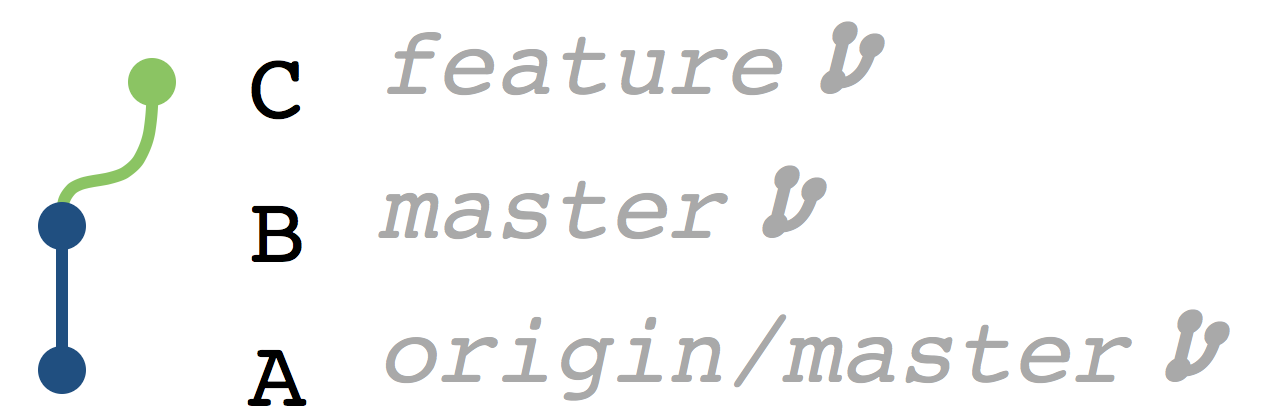
\includegraphics[width=\textwidth]{Figures/background/foxtrot/step_1.png}
    \caption{The initial local repository.
      The origin master branch is on commit A.
      The local master branch on commit B, and the feature branch on commit C.}
  \end{subfigure}
  \begin{subfigure}[b]{0.3\textwidth}
    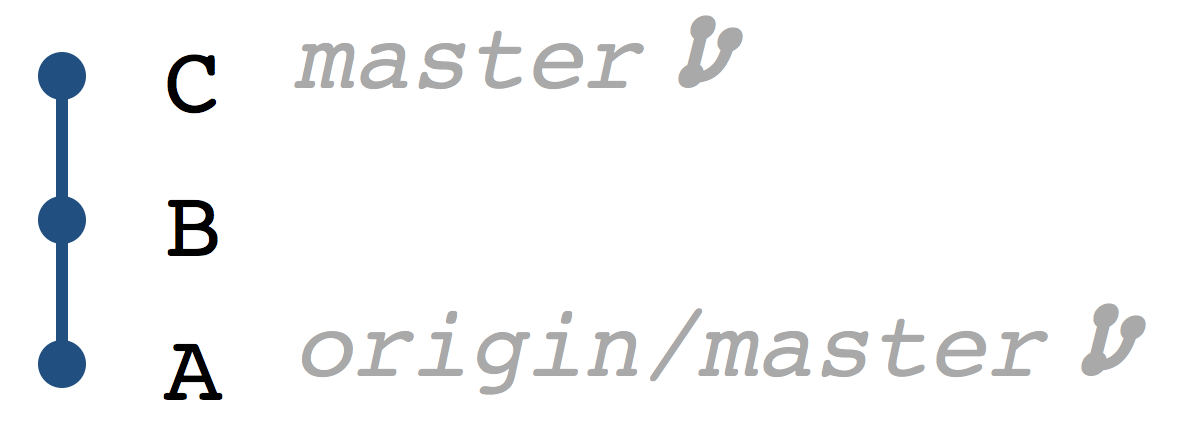
\includegraphics[width=\textwidth]{Figures/background/foxtrot/step_2.png}
    \caption{We perform a fast-forward merge bringing C into the local master branch.}
  \end{subfigure}
  \begin{subfigure}[b]{0.3\textwidth}
    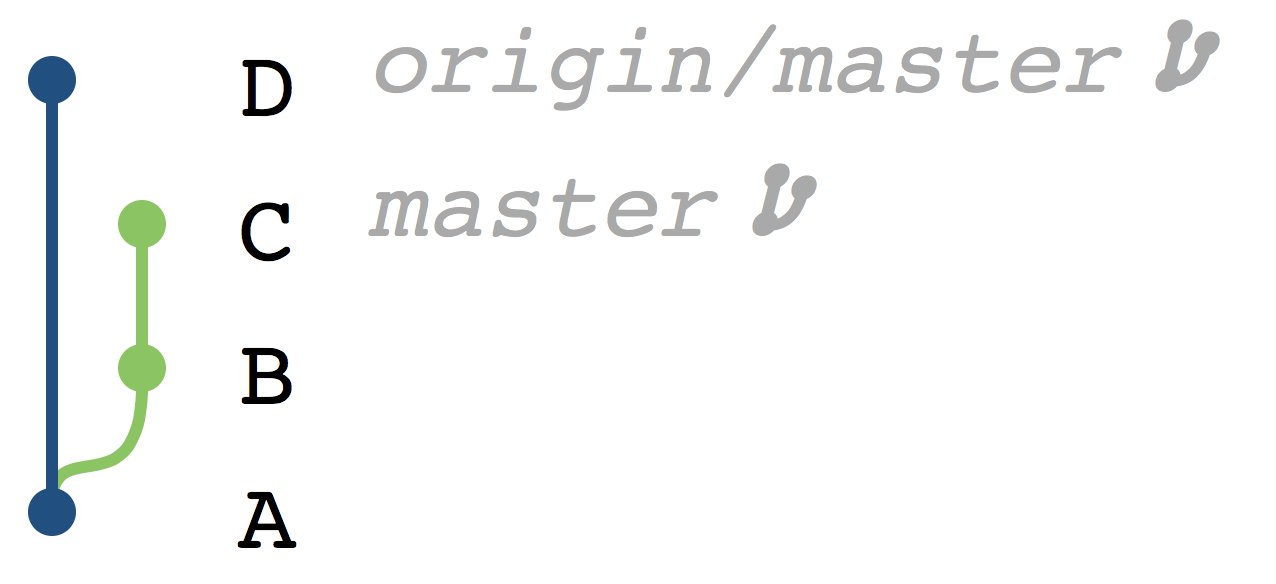
\includegraphics[width=\textwidth]{Figures/background/foxtrot/step_3.png}
    \caption{Meanwhile, Commit D is committed and pushed to the master
      branch of the master repository.}
  \end{subfigure}

  \begin{subfigure}[b]{0.3\textwidth}
    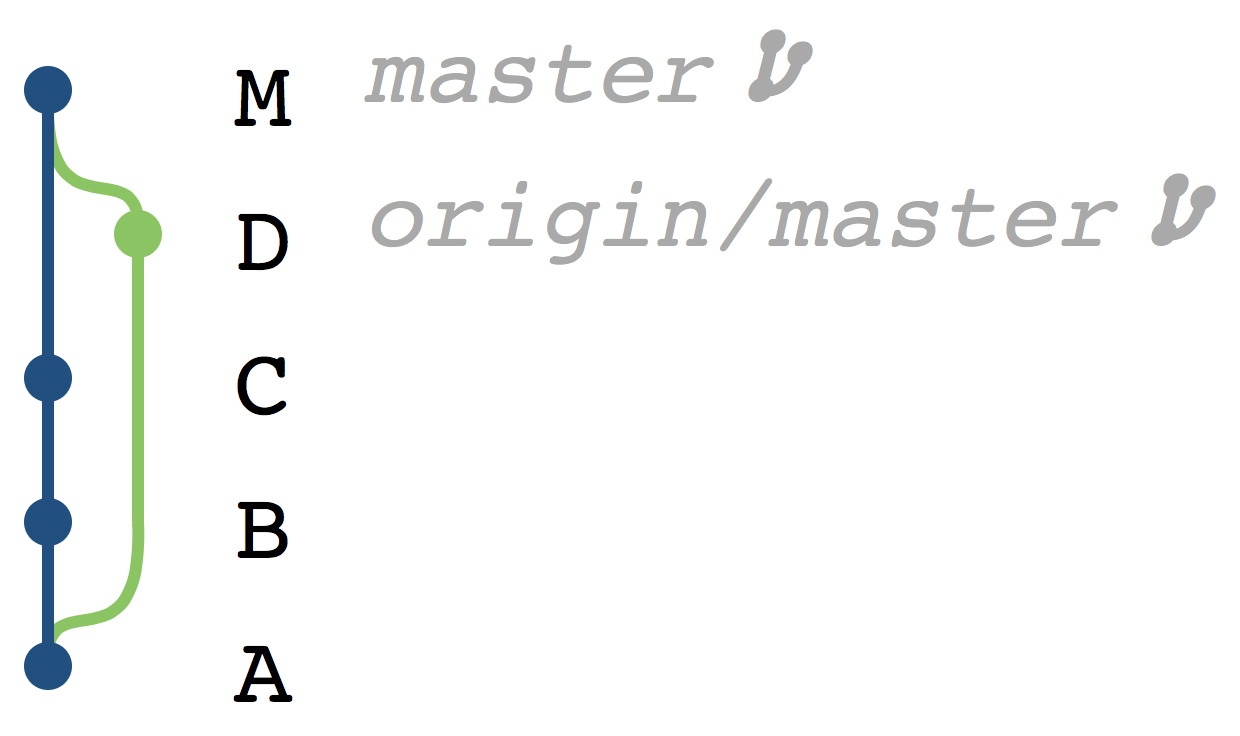
\includegraphics[width=\textwidth]{Figures/background/foxtrot/step_6.png}
    \caption{Pulling directly will merge the master branch of the master
      repository into the master branch of the local repository.}
  \end{subfigure}
  \begin{subfigure}[b]{0.3\textwidth}
    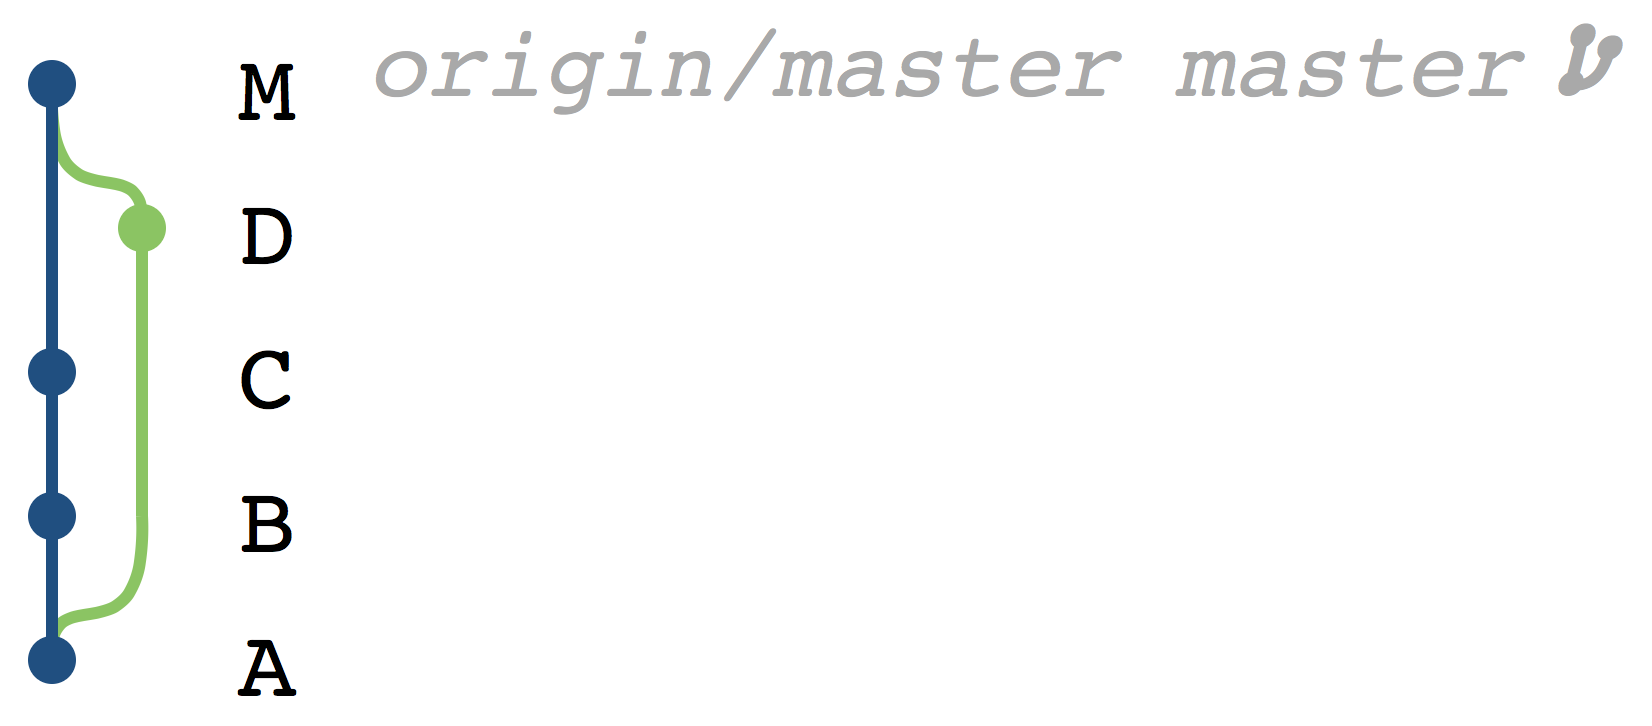
\includegraphics[width=\textwidth]{Figures/background/foxtrot/step_7.png}
    \caption{Pushing the change into the master repository completes the
      steps of the foxtrot. Commit D started on the master branch of the
      remote repository, but appears to be on a separate branch due to
      the flip that occurred when the pull was made.}
  \end{subfigure}

  \caption{This series of figures show the steps to create a foxtrot.
    The foxtrot occurs when the remote master branch is merged into the
    local master branch instead of the local branch being merged into
    the remote branch.}
  \label{fig:foxtrot_steps}
\end{figure}

As a convention, the first parent of a node is on the same branch as
that node.
A\foxtrot\footnote{See \url{http://bit-booster.blogspot.ca/2016/02/no-foxtrots-allowed.html} for a full description of the issue.}
merge occurs when the order of the parents is changed, confounding the
branch relationship (depicted in Figure~\ref{fig:foxtrot_steps}).

Foxtrot merges are created when the developer pushes their changes to
the remote repository.
Prior to pushing, the developer will perform a pull, which synchronizes
their local repository with the remote repository.
If there are no conflicts between the local and remote repositories, the
merge is fast-forwarded and no merge commit is created.
When the developer pushes their changes, the local repository is merged
into the remote repository.
This results in a fast-forward merge, there will be no merge conflicts
because these were corrected in the pull.
If a conflict should arise, the remote repository will reject the push.
If there is a conflict when the developer pulls, the developer must
correct the conflicts.
These corrections are stored in the merge commit, which merges the
remote repository into the local repository.
The creation of this merge commit is the first step in creating the
foxtrot.
The first parent of the merge commit will be the commit on the local
branch, not the head of the remote repository.
When the changes are pushed back to the server, the master branch of the
remote repository changes from the original head prior to the merge to
the merge commit, which flips the branches.
The end result is that the commits that were made to the developer's
local branch are shown as the commits to the master branch of the remote
repository.

This confounds the true master coming from the remote repository with
the master branch in the local repository; the commits in the local
repository appear as the commits added to the master branch, while the real
master branch appears to be a branch merged into the local repository.

The nodes in the DAG are immutable; once a commit or merge is created,
it cannot be changed. Git allows operations to alter the events and
re-order them, but this will create a new event with a new commit hash.
This property makes it impossible for nodes to store information about
the children, and in extension, how the commit is being merged as this
information is not available when the commit is created.
Git provides the command \verb|git log --children|, which traverses the
DAG and inverts the edges.
The goal is to identify the series of merges that a commit takes to
reach the master branch.
The next child that is a merge is the first merge on the path to being
integrated.

The graph combined with the child information gives most of the
information necessary for understanding how the commit is
merged into the master branch; however, it is missing which merge is
into the master branch, and the information is not always easy to
understand, as shown in Figure~\ref{fig:git_graphs}.

\begin{figure}[htpb]
  \centering
  \begin{subfigure}[b]{0.8\textwidth}
    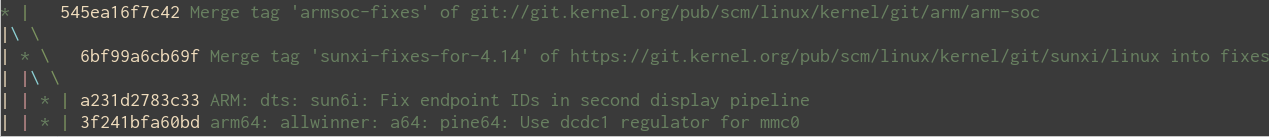
\includegraphics[width=\textwidth]{Figures/background/git_graph.png}
    \caption{In the simple case, it is relatively easy to see
      that \textit{a231d} is merged into \textit{6bf99},
      which is then merged into \textit{545ea}.}
    \label{fig:trivial_graph}
  \end{subfigure}

  \begin{subfigure}[b]{0.8\textwidth}
    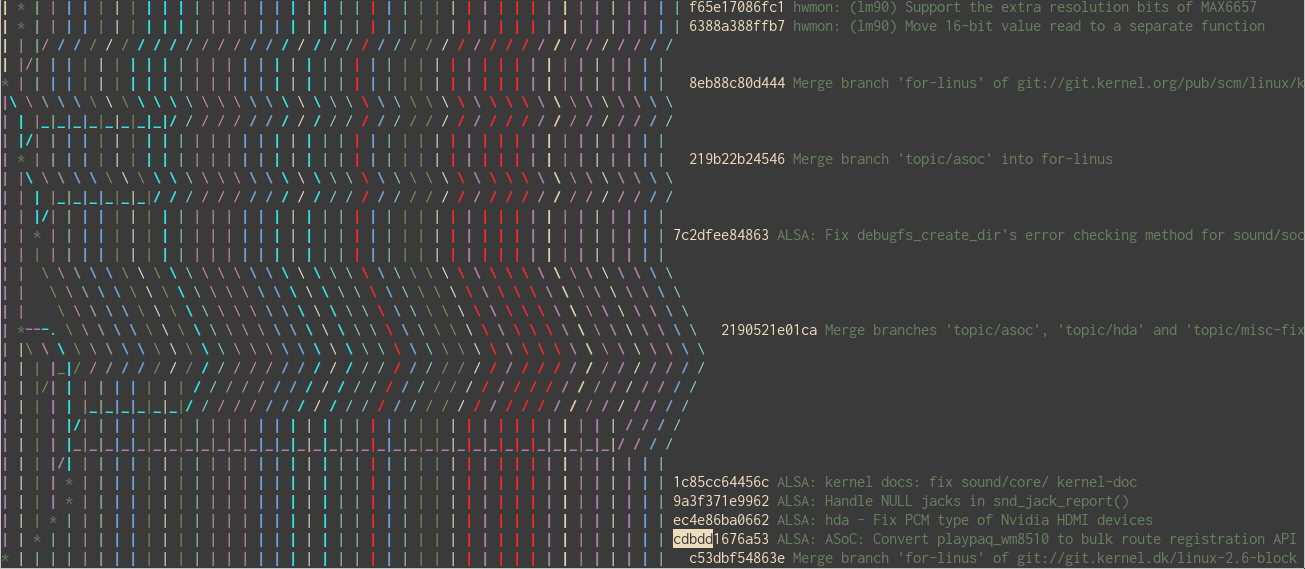
\includegraphics[width=\textwidth]{Figures/background/git_graph_complex.png}
    \caption{As the number of merges that a commit passes through
      increases, it becomes more challenging to understand how the
      commit is integrated.}
  \end{subfigure}
  \caption{The git graph visualization of two sections of the Linux
    repository.}
  \label{fig:git_graphs}
\end{figure}

Most repositories are simple enough that it is possible to identify how
commits are integrated using the visualizations of the DAG that are
available with the current tools. Difficulties arise in larger
repositories. The master branch can be confounded with \foxtrot{}
merges, making it difficult to identify. Sheer number of commits being
added to various branches at a given time can make it difficult to
understand which branch a commit is being added to.

\section{Linux}\label{sec:linux}

This \paper{} studies and proposes a visualization for the Linux kernel
repository.
The repository itself is complex, contain tens of thousands of commits
and thousands of merges per year.
Older versions of the kernel are used in a wide
variety of situations including various Linux desktop distributions,
internet of things device firmware, web servers,
spacecrafts\footnote{Linux is used heavily at SpaceX
  \url{https://lwn.net/Articles/540368/}}, and in mobile devices as the
base of the Android platform. These kernels are sometimes modified forks
of the official Linux kernel, made to be more suitable for the specific
needs of the application. Due to these application-specific
modifications, it is not feasible to update to the latest version of the
kernel. While it may not be feasible to update, the changes being made
to the official version are necessary as they fix bugs, patch security
issues, and improve performance. Due to the sometimes critical nature of
the patches being merged into the current version of the kernel, it is
necessary for maintainers working on an application-specific fork of the
kernel to sift through the commits coming into the official version,
looking for changes that may impact the kernel that they are
maintaining.
This section presents statistics on the dataset collected from the Linux
repository. Included is information about the number of authors,
commits, and merges per release, as well as the range of dates from
which the data was collected. This information is useful for
characterizing the problem, and understanding how to best group the
commits in a way that is useful and easy to understand.

The data extracted from the repository involves all merges into the
master branch between April 18, 2005 and August 14, 2014. This
corresponds to the merges added to the kernel between versions 2.6.11
and Linux 3.16.
The commits collected from the repository include commits authored
between September 17, 2001 and December 6, 2014.
There are 4 commits in the dataset that are beyond this range due to
the date being incorrectly set on that developer's machine.
There is one incorrect date that is dated January 1, 1970, authored by
Ursula Braun, and three commits dated after 2014.
These commits are dated April 5, 2019, October 14 2030, and
April 25 2037, authored by Len Brown, Yanmin Zhang, and Daniel Vetter,
respectively.
Commits are not necessarily merged immediately, all commits were added
between April 15, 2005 and October 14, 2014.
This breakdown of the kernel data focuses on the commits integrated
into kernel versions Linux 3.1 to Linux 3.16, translating to the merges
between July 21, 2011 and August 3, 2014.

As expected, the Linux kernel is highly collaborative and is very
active. Between 1000 and 1500 authors have contributions accepted into
the official kernel per release (shown in
Figure~\ref{fig:linux_authors_per_release}). These authors contribute
between 8000 and 14000 commits per release
(Figure~\ref{fig:linux_commits_per_release}). Between 275 and 400 merges
integrate the commits into the master branch of the kernel per release
(Figure~\ref{fig:linux_commits_per_release}). The Linux kernel
repository is a prime example of a successful open source project,
exemplifying the collaborative nature of modern software development.
The sheer number of commits being contributed make the task of filtering
the important or relevant commits impractical.

\begin{figure}[htpb]
  \centering
  \includegraphics[width=0.8\linewidth]{Figures/background/linux_authors_per_release.pdf}
  \caption{Unique authors with contributions to each kernel version}
  \label{fig:linux_authors_per_release}
\end{figure}

\begin{figure}[htpb]
  \centering
  \includegraphics[width=0.8\linewidth, page=1]{Figures/background/linux_commits_per_release.pdf}
  \caption{Commits per release from Linux 3.1 to Linux 3.16}
  \label{fig:linux_commits_per_release}
\end{figure}

\begin{figure}[htpb]
  \centering
  \includegraphics[width=0.8\linewidth, page=2]{Figures/background/linux_commits_per_release.pdf}
  \caption{Merges per release from Linux 3.1 to Linux 3.16}
  \label{fig:linux_merges_per_release}
\end{figure}

While the number of integrating merges into the master branch appears to
be decreasing slightly per release, the number of commits per release is
increasing.
The average (mean) number of commits per merge per release has
increased from slightly over 20 commits per merge into the master branch
in Linux 3.1 up to 50 commits per merge in Linux 3.16
(Figure~\ref{fig:linux_commits_per_merge_per_release}).

\begin{figure}[htpb]
  \centering
  \includegraphics[width=0.8\linewidth, page=3]{Figures/background/linux_commits_per_release.pdf}
  \caption{Commits per merge into each release of Linux from 3.1 to 3.16}
  \label{fig:linux_commits_per_merge_per_release}
\end{figure}

Grouping the commits by the merge that integrates int into the master
branch and taking the median number of commits per merge shows a
different view of the kernel repository.
The individual merges contain
relatively few commits, 25\% of the merges merge only a single commit,
and 50\% of the merges merge at most 7 events
(Figure~\ref{fig:linux_merge_distribution_per_release}).

\begin{figure}[htpb]
  \centering
  \includegraphics[width=0.8\linewidth]{Figures/background/linux_merge_distribution_per_release.pdf}
  \caption{Distribution of Merge Sizes per Release Between Linux 3.1 and
  3.16}
  \label{fig:linux_merge_distribution_per_release}
\end{figure}
